%% ID: pulleys_on_table
%% TITLE: Pulleys on a Table
%% TYPE: question
%% QUESTIONTYPE: symbolic
%% CONCEPTS: energy, momentum, eq_of_motion_diff, newtonii, impulse
%% VIDEOS: 
%% LEVEL: 3
%% TOPIC: mechanics/dymanics
%% ORDER: 10

\begin{problem}[A1969AMIIQ2a] %Slightly tricky impulse, energy and SUVAT question
{\begin{figure}[h]
\centering
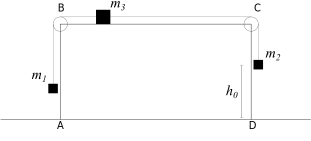
\includegraphics[width=0.5\textwidth]{../../../figures/Dynamics_table_pulley_masses.eps}
\caption{}\label{fig:Dynamics_table_pulley_masses}
\end{figure}

Figure \ref{fig:Dynamics_table_pulley_masses} shows the cross section of a smooth table ABCD, standing on the floor AD, with smooth pulleys attached at B and C. Particles of masses $m_{1} < m_{2} < m_{3}$ are attached to a light, inelastic, inextensible string which passes over the pulleys as shown. The system is released from rest with the string taut when $m_{2}$ is a height $h_{0}$ from the floor.
\begin{enumerate}
	\item Find the initial acceleration of the system.
	\item The mass $m_{2}$ hits the floor. Describe the subsequent motion of the system until the string again becomes taut. Find the following quantities, given that $m_{1} = 1$ kg, $m_{2} = 3$ kg, $m_{3} = 5$ kg and $h_{0} = 0.45$ m:
	\begin{enumerate}
		\item the velocity with which the system will move just after the string again becomes taut,
		\item the impulse on $m_{2}$ at this instant, and the resulting loss of kinetic energy.
	\end{enumerate}
	\item Show that, when the system next comes instantaneously to rest, $m_{2}$ will be $\frac{4}{9}h_{0}$ above the floor.
\end{enumerate}
[You may assume that, during the motion, none of the masses come into contact with a pulley.]
}
{\textit{Adapted with permission from UCLES, A Level Applied Mathematics, June~1969, Paper~2, Question~2.}}
{\begin{enumerate}
	\item Since $m_{2} > m_{1}$, the masses will start to move clockwise with an acceleration given by Newton's Second Law. The total force on the string is $(m_{2} - m_{1})g$ and so we obtain:
	\begin{align*} F &= (m_{2} - m_{1})g\\ &= (m_{1} + m_{2} + m_{3})a \end{align*} so \begin{align*} a = \frac{(m_{2} - m_{1})g}{m_{1} + m_{2} + m_{3}} = a_{0} \end{align*}
is the initial acceleration.
	\item It is best to leave everything in symbols until the very end of the solution:
	\begin{enumerate}
		\item This step can be simplified by a realisation based on energy principles. When $m_{2}$ hits the floor there is no longer any tension in the string, but the other two masses have momenta that will carry them onwards and make the string slack. But $m_{1}$ now has a net force of $-m_{1}g$ acting on it, which will slow both masses and reverse their motion. When they get back to the point they were at as $m_{2}$ hit the ground, the string will go taut again. Since the surface is smooth the kinetic energy of $m_{1}$ and $m_{3}$ must be the same as it was initially; there are no losses to friction and the gravitational potential energy is unchanged. Thus the speed of $m_{1}$ and $m_{3}$ the instant the string goes taut must be the speed the masses were moving at as $m_{2}$ hit the ground.

This can be found by using the SUVAT equations, since the masses move together from rest at a constant acceleration. We want to use the equation $v^{2} = u^{2} + 2as$, where $s = h_{0}$, $u = 0$ and $a = a_{0}$:
\begin{align*} 
v &= \sqrt{u^{2} + 2as} = \sqrt{(0)^{2} + 2(a_{0})(h_{0})} = \sqrt{2a_{0}h_{0}} \\
 &= \sqrt{2\left(\frac{(3 - 1)(9.8)}{1 + 3 + 5}\right)(0.45)} \text{ ms}^{-1} = \frac{7}{5} \text{ ms}^{-1} = 1.4 \text{ ms}^{-1}  
 \end{align*}
which is the speed they must be moving at as the string goes taut once more. 

This can be shown another way; by using SUVAT again, if the energy reasoning is unclear or just as a check. The mass $m_{1}$ has a force $-m_{1}g$ acting on it and so the tension in the string must equal this too, giving $m_{1}$ and $m_{3}$ together an acceleration of $a_{c} = \frac{-m_{1}g}{m_{1} + m_{3}}$. Then we use the same SUVAT equation as before, but now $s = 0$ in order that the string go taut again; the displacement is zero since they return to the same position, and $a = a_{c}$:
\begin{equation*} 
v = \sqrt{u^{2} + 2as} = \sqrt{u^{2} + 2a_{c}(0)} = \sqrt{u^{2}} = u 
\end{equation*}
so the masses have the same speeds as initially; as expected from the energy reasoning.

This is not the final answer, since just after the string goes taut $m_{2}$ will be moving as well. To find the final speed, $w$, all three masses have immediately after the string goes taut, conserve momentum:
\begin{align*} 
(m_{1} + m_{3})(v) + (m_{2})(0) = (m_{1} + m_{2} + m_{3})(w) 
\end{align*}
\begin{align*}
 w = \frac{m_{1} + m_{3}}{m_{1} + m_{2} + m_{3}} v 
 \end{align*}

		\item The impulse on $m_{2}$ is simply the change in its momentum as it is lifted from the floor. It starts stationary on the floor and is then moving upwards at a speed $w$:
\begin{align*} 
I &= (m_{2})(w) - (m_{2})(0) = m_{2}w = \frac{m_{2} \left(m_{1} + m_{3} \right)}{m_{1} + m_{2} + m_{3}} v = \frac{m_{2} \sqrt{2a_{0}h_{0}} \left(m_{1} + m_{3} \right)}{m_{1} + m_{2} + m_{3}} \\ 
&= \frac{(3)(1.4)(6)}{9} \text{ kg ms}^{-1} = \frac{14}{5} \text{ kg ms}^{-1} = 2.8 \text{ kg ms}^{-1}
\end{align*}

The loss in kinetic energy (KE) as $m_{2}$ starts moving is given by the total KE before, minus the KE after:
\begin{align*} 
\text{KE Loss} &= \left( \frac{1}{2}m_{1}v^{2} + \frac{1}{2}m_{3}v^{2} \right) - \left( \frac{1}{2}m_{1}w^{2} + \frac{1}{2}m_{2}w^{2} + \frac{1}{2}m_{3}w^{2} \right) \\ 
&= \frac{1}{2} \left( (m_{1} + m_{3})v^{2} - (m_{1} + m_{2} + m_{3})w^{2} \right) \\ &= \frac{1}{2}v^{2} \left( (m_{1} + m_{3}) - \frac{(m_{1} + m_{3})^{2}}{m_{1} + m_{2} + m_{3}} \right) \\ 
&= \frac{1}{2}(1.4)^{2} \left( 6 - \frac{36}{9} \right) \text{ J} \\ 
&= \frac{49}{25} \text{ J} = 1.96 \text{ J}
\end{align*}
	\end{enumerate}
	\item The masses are now moving anticlockwise around the edge of the table but have the initial, clockwise, force acting on them. Thus they have a constant deceleration and will come to instantaneous rest. The SUVAT equation $v^{2} = u^{2} + 2as$ can be used to find $h$, the height $m_{2}$ reaches above the floor before it stops. Using $s = h$, $u = w$, $v = 0$ and $a = -a_{0}$:
\begin{align*}
 h &= \frac{v^{2} - u^{2}}{2a} = \frac{-w^{2}}{-2a_{0}} = \left( \frac{m_{1} + m_{3}}{m_{1} + m_{2} + m_{3}} \right)^{2} \left( \frac{v^{2}}{2a_{0}} \right) =  \left( \frac{m_{1} + m_{3}}{m_{1} + m_{2} + m_{3}} \right)^{2} h_{0} \\ 
 &= \left( \frac{6}{9} \right)^{2} h_{0} = \frac{4}{9} h_{0}
 \end{align*} 
 as required.
\end{enumerate}}
\end{problem}